\chapter{Keyframes}%
\label{cha:keyframes}

The word \textit{keyframe} has at least 3 contextual meanings in the NLE environment.  First, the oldest meaning, is the \textit{I-Frame} definition used in codecs algorithms.  These are \textit{key} frames that begin a new sequence of pictures, and are anchor points for repositioning (seeks).  Next are the automation parameter data points.  These are usually input to primitive math forms, like translation and zoom.  And last are blobs of data that are chunks of parameters to plugins that can do almost anything.  The data can be a simple value, like a fader value, or more complex like a group of points and colors in a sketcher plugin keyframe.  The word keyframe has changed a lot in meaning.  In the context of Cinelerra, keyframes are data values that have been associated to the timeline which affect the media presentation.  So a keyframe no longer refers to a frame, but to a position on the timeline.

In Cinelerra, there are two general types of keyframe data, \textit{automation keyfra\-mes} (autos) which are drawn as colored lines and box icons overlayed at a point on a media track, and \textit{plugin keyframes} which are drawn as gold key symbols on a plugin bar of a track.  \quad
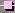
\includegraphics[height=\baselineskip]{images/auto.png}	         
Auto $\leftarrow$ Keyframe $\rightarrow$ 
Plugin 
\includegraphics[height=\baselineskip]{images/plugin.png}

\section{Automation Keyframes / Autos}%
\label{sec:automation_keyframes_autos}

The \textit{autos} are created by clicking on an \textit{automation curve} to establish the time position for the new keyframe anchor point.  The basic nature of these simple auto values make them primitive operations that are easy to apply when needed.  

There are many automation curve types, and most are not normally visible or clickable.  To make them visible, use the \textit{View} pulldown, or open the \textit{Show Overlays} window in the \textit{Window} menu pulldown.   This window allows toggling of the parameters in the View pulldown but is more convenient because you can leave the window up to change values quickly.  If all of the automation curves are turned on, the timeline will be quite cluttered, and so usually only the parameters of interest are enabled during use.  When keyframes are selected, they are drawn on the timeline over the tracks to which they apply.  The keyframe is represented on the timeline as a little square on the curve, for example as in fade, or as a symbol as in a mask.  This square, timeline attachment point, can be used for positioning by clicking on a keyframe anchor and using drag and drop to set the new position.

The automation keyframes include:

\texttt{mute/play audio}, \texttt{camera translation x,y and zoom}, \texttt{projector\\
    translation x,y and zoom}, \texttt{fade blending}, \texttt{audio panning}, \texttt{overlay mode}, \texttt{mask point sets}, and \texttt{sampling speed} 

Except for the mask auto, the values are all simple numbers.  Mute is different from the other autos in that it is simply a toggle of either on or off.  Mute keyframes determine where the track is processed but not rendered to the output.  An example usage would be to use auto keyframes to fade in a clip by setting the transparency to $100\%$ at the first keyframe and adding another keyframe 5 seconds later in the timeline with a transparency of $0\%$.  

The Keyframes pulldown on the main timeline is used for Cut, Copy, Paste, Clear, Change to linear, Change to smooth, Create curve type of Smooth, Linear, Tangent, or Disjoint, Copy default keyframe or Paste default keyframe.  If you right click on a curve keyframe on the timeline, a set of options popup including the choices \textit{keyframe type} (such as Fade, Speed, etc.), Hide keyframe type, Delete keyframe, Copy keyframe, smooth curve, linear segments, tangent edit, or disjoint edit.

Usually, the use of the keyframe values are more pleasing when the data varies smoothly between keyframe anchors on the timeline.  This is useful in many cases that are familiar, like a video fade in/out, or audio pan between channels.  To make the auto value change smoothly as the media is played, the keyframes auto values are points on curves that are created according to the design of the effect.  Most of the primitive types can create anchor points on curves that are piecewise linear, smooth, sloped, or broken at the keyframe anchor points.

Curve smoothing is called \textit{interpolation} and it uses keyframe point values and control values that determine how the curve will react at the time the media is played or rendered.  Interpolation uses 2 keyframes to create a set of intermediates which are used as active values between the \textit{previous} and \textit{next} keyframe anchors on the timeline.  The way the intermediate data is generated depends on the type of curve used to invent these values.  Cinelerra interpolates the intermediate values making the change happen smoothly and gradually over time.  The simple linear mathematical formula for interpolation is:   $a\times(1-t) + b\times t$    where $0\le t\le 1$ uniformly.

\section{Using Autos}%
\label{sec:using_autos}

The first click on the curve, creates a keyframe which you can \texttt{click drag} on to reposition.  The second click at a later position, generates the smoothing by creating a smooth ramp.  \texttt{Ctrl-dragging} on a keyframe round control point handle changes the value of either the input control or the output control.  This affects the sharpness of the curve.  While the input control and the output control can be moved horizontally as well as vertically, the horizontal movement is only for legibility and is not used in the curve value.  When you \texttt{Shift-drag} on a timeline curve, the keyframe snaps to the value of either the next or previous keyframe, depending on which exists.  It will snap up or down depending on direction of movement.  This lets you set a constant curve value without having to copy the next or previous keyframe.

To make it easier to navigate curve keyframes, since there is not much room on the timeline for a wide range of curve values, you need to zoom the curves in and out vertically to have any variability.  This is done by 2 tools: the automation fit button, \texttt{Alt-f}, and automation zoom menu which is seen at the bottom of the main window (figure~\ref{fig:automation}). The automation fit button scales and offsets the vertical range so the selected curve area appears in the timeline.  If a region of the timeline is highlighted by the cursor, only that region is scaled.  In/out points do not affect the zoomed region.  The automation zoom menu manually changes the vertical scaling of the curves in multiples of 2.  Click on its tumbler to change the zoom.  \texttt{Alt-up arrow} and \texttt{Alt-down arrow} change the automation zoom from the keyboard.

\begin{figure}[htpb]
    \centering
    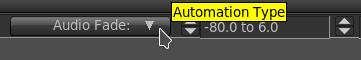
\includegraphics[width=0.7\linewidth]{images/automation.png}
    \caption{Automation zoom menu with tumbler}
    \label{fig:automation}
\end{figure}

\noindent Other mouse actions have the following effects:

\begin{itemize}
    \item Double left mouse click on a curve Fade or Speed line will create ganged keyframes so that there is a
    keyframe on each of the tracks in the exact same position.
    \item Left mouse click on a keyframe position will show the numerical value in a yellow tooltip-like box.
    \item Right mouse click on the curve type line will bring up the option of \textit{Hide keyframe type}.   This
    provides the same functionality as disabling the keyframe type in the View pulldown menu.  Often it
    helps to use this in order to be able to see other things on the timeline once it gets cluttered.
    \item Fade and speed allow for setting a specific value for the keyframe using the following:
    \begin{enumerate}
        \item click using the right mouse button on one of the auto speed keyframes on the timeline;
        \item a popup menu comes up with speed or fade auto type as the first menu item;
        \item click on speed or fade and a colored slider bar will appear (default speed=orange; fade=pink);
        \item click the slider, press and hold the left mouse button and move the slider to update the value or
        simply type in a value in the textbox followed by pressing the Enter key or click the checkmark;
        \item a tooltip shows the keyframe value;
        \item release the button, the slider will be deleted from the canvas, and the value will be updated.
    \end{enumerate}
\end{itemize}

You can click mouse button 3 on a keyframe box and a menu pops up with the first menu item showing the keyframe type.  The top menu item can be activated for immediate access to update the automation keyframe value.  Some keyframe types, which have values that can be manipulated in another way than by dragging the color coded line, now show up with a different colored background to make them more visible.  Keep in mind that Zoombar ranges/values must be set to appropriate values when working with specific keyframe types, such as Fade or Speed.  If you do not see the auto line in the visible area of the video track, try the key combination \texttt{Alt-f} or select the speed in the \textit{Automation Type} drop-down menu at the bottom of the main window.  To the right of this field is \textit{Automation Range} where you can set the display ratio of these lines. Simply change the values until the lines are visible again. 

Figure~\ref{fig:overlays1} and figure~\ref{fig:fade} shows several color coded lines for different key\-fra\-mes and specifically the slider bar for the Fade keyframe.  It is in the same color as the color coded keyframe type line which is the same color which would be shown in the \textit{Show overlays} window figure~\ref{fig:overlays_window}.

\begin{figure}[htpb]
    \centering
    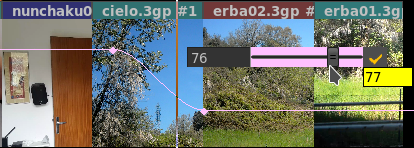
\includegraphics[width=0.8\linewidth]{images/fade.png}
    \caption{Fade curve with pink colored box Keyframe and Slider bar}
    \label{fig:fade}
\end{figure}

In the \textit{Editing} section of \texttt{Settings $\rightarrow$ Preferences}, the Interface tab there is \textit{Keyframe reticle} with options of Never, Dragging, or Always.  This is used to help in checking edit alignment across tracks.  (A reticle is a sighting line used to line up visual items, like cross hairs in a eyepiece.)  The appearance and function of sighting lines can be changed when dragging auto keyframes.  To see the effect, create some fader autos and drag a few to see the reticles drawn --- you will see something similar to the next screencast (figure~\ref{fig:always}).  \textit{Always} renders a line over all plugins, and \textit{dragging} only over the drag icon. \textit{Never} draws nothing.  The default is \textit{dragging}.

\begin{figure}[htpb]
    \centering
    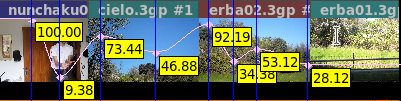
\includegraphics[width=0.8\linewidth]{images/always.png}
    \caption{Fade Auto with \textit{Always} set for easy to see numeric values}
    \label{fig:always}
\end{figure}

\begin{wrapfigure}[9]{O}{0.5\linewidth}
    \vspace{-2ex}
    \centering
    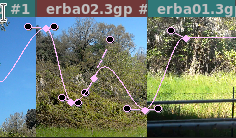
\includegraphics[width=0.79\linewidth]{images/controls.png}
    \caption{Fade Auto with Controls}
    \label{fig:controls}
\end{wrapfigure}

Control points allow for setting the slope of auto curves and then
subsequently adjusting that slope (figure~\ref{fig:controls}).  To modify a current keyframe
you just right mouse it and change to either Tangent or Disjoint edit.
In the screencast to the right, the Fade Auto has pink colored curves and control points are seen as dashed lines next to the keyframe box with black filled circles on each end of the line.  Use the Ctrl key with the left mouse button to modify the control point lines.

\section{Speed / Fade Automation Usage and Auto Gang}%
\label{sec:speed_fade_automation_gang}

Speed automation resamples the data at a higher or lower playback rate. Speed automation can operate
on all tracks of the same type, either video or audio, with a single click; or all tracks, both video and
audio, with a double click. The curves to be affected must be both armed and ganged in the track
patchbays to be included in the operation. You can see the advantage of having different media types
ganged the same so that they will remain synchronized.  However, if as recommended you have Settings of \textit{Align cursor on frames} set, video will always snap to a frame, whereas audio does not.  Because the smallest pieces are audio and not video, when video is present in order to maintain synchronization be sure to do the double click on the video track.  The single/double click feature also works in the same manner for Fade Automation.

The conversion algorithms that calculate the duration are approximate, not exact.   Speed is not checked when inserting media on a track that already has speed adjustments so duration will not be corrected in that case.  You can not do negative time and you can not play backwards.

Steps to demonstrate Auto Gang of Speed/Fade on all of the audio and video tracks are listed below:

\begin{enumerate}
    \item Use the pulldown menu \textit{View} on the main canvas and ensure that there is a checkmark left of the Speed or Fade selection.
    \item Double click and hold button 1 on any point of the Speed line on any track of the main track canvas and drag the handle where you want it, then release button 1.
    \item Note how all video and audio boxes move together simultaneously for synchronization.
    \item You can adjust the sampling rate (speed/fade) at any time by doing the same single/double
    click on a keyframe.
    \item To move the location left or right, hold down button 1 while moving it back and forth.
    \item Use the status bar in the lower left hand corner to see position and playback rate.
\end{enumerate}

Releasing button 1 ends the current dragging operation, but single clicking on a speed/fade keyframe handle again will restart the drag operation on tracks of the same type.  Double clicking will select all armed tracks which have handles in the exact same cursor position.  It is sometimes difficult to get the desired value for the speed and it may take a few tries to get to the desired endpoint, but you can use an auto slider bar to get better control for more precision.  This is not ganged so you will have to do this on each track to achieve the same value.

An easy way to get an exact position is to set the "Automation range" in the bottom bar of the main
window to the low and high ends of the desired range. For example, 1.000 to 50.000, which makes it
so you can drag the speed/fade handle all the way to the left for 1.000 or all the way to the right for 50.

Figure~\ref{fig:always} shows orange keyframes and lines for the ganged speed automation on all video/audio tracks.
Note the status bar numbers in the lower left-hand corner displaying 2.17 seconds as the location and 0.38 as the playback rate. The figure also shows the orange speed slider bar triangle with the current value displayed via the tooltip.

\begin{figure}[htpb]
    \centering
    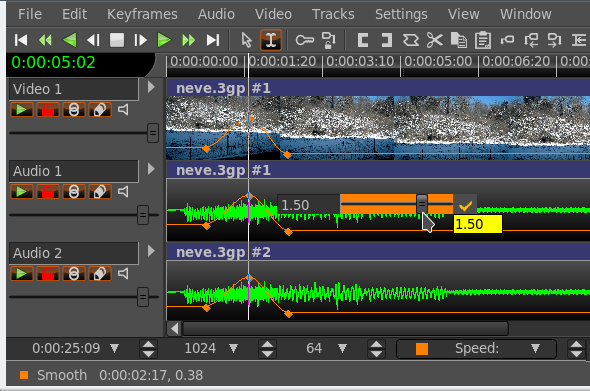
\includegraphics[width=0.8\linewidth]{images/speed.png}
    \caption{Ganged Speed Auto on all tracks and Speed auto with orange Slider bar}
    \label{fig:speed}
\end{figure}

One other helpful item is a small colored indicator in the zoombar \textit{Automation Type} box when you have clicked on an auto line.  It will be the same color as that line so you can easily see out of the corner of your eye what that line refers to.  This is especially useful for the Camera and Projector X,Y,Z lines which are often right on top of each other.  In addition the status bar will have the colored indicator to the left of the last auto value when that status is visible.

\section{Plugin Keyframes}%
\label{sec:plugin_keyframe}

The Plugin keyframes are structured.  The individual data values are named parameters to the keyframe function.  For example, the hue plugin has keyframe parameters of hue, saturation, and value.  Each plugin has its own parameters, and what they do depends on the plugin.  Most of the time, it is pretty obvious what the value controls, like the audio gain plugin with the level parameter.  Some of the plugins have a wide variety of controls, like the titler which can setup a wide number of controls, like formats, fonts, styles, placement, and so on.

Plugins also may use interpolation to smooth the data between the keyframe paramaters on the timeline.  Just exactly how this is done varies with the plugin and is not always easy to predict, but this
is usually due to the nature of the keyframe parameter data.  For example, it does not make sense to interpolate which font is in use.

\section{Default Keyframe}%
\label{sec:default_keyframe}

For plugins, there is a special hidden keyframe, called the \textit{default keyframe}, that is used when no previous keyframe exists.  It is like keyframe zero on the timeline, and it is persistent and shared on
all sessions.  The intent is to make a parameter set that is likely to be reused on all initial instances of the plugin.  An example may be to color correct a set of media that was taken in low light, or needs resampling to be played correctly.  The default keyframe is \textit{off the bar on the left side} of the plugin title bar and can not be seen.  It is used when there is no \textit{previous} keyframe for its default values.

It may be useful to create a default keyframe which has specific desirable values for later use.  To do this, set the timeline to position 0 and be sure to disable \textit{generate keyframes while tweaking}.  This will create a default keyframe at the beginning of the timeline which contains global parameters for the entire duration.  Or if you have copied a non-default keyframe via Keyframes pulldown \textit{copy default keyframe}, it can be stored as the default keyframe by calling \texttt{keyframes$\rightarrow$paste default keyframe}.  After using paste default keyframe to convert a non-default keyframe into a default keyframe, you will not see the value of the default keyframe reflected until all the non-default keyframes are removed.

The \texttt{keyframes$\rightarrow$copy default keyframe} and \texttt{keyframes} $\rightarrow$ \texttt{paste} {\texttt{de\-fault keyframe} allow conversion of the default keyframe to a non-default key\-fra\-me.

\texttt{Keyframes$\rightarrow$copy default keyframe} copies the default keyframe to the clipboard, no matter what region of the timeline is selected.  
The \texttt{keyframes}$\rightarrow$ \texttt{pas\-te} \texttt{keyframes} function may then be used to paste the clipboard as a non-default keyframe.  

\textit{Typeless keyframes} enabled under the Settings pulldown allow keyframes from any track to be pasted on either audio or video tracks.  Ordinarily audio keyframes can only be pasted to another audio track and video keyframes can only be pasted to another video track.

\section{Keyframe \textit{Edit Params} for Plugins}%
\label{sec:keyframe_edit_params_plugin}

Keyframe values can be set using the various plugin \textit{show controls} (magnifying glass) icon on the plugin track (figure~\ref{fig:parameters}).  It is possible to see all of the keyframe data in a raw format using the \textit{Edit Params} popup menu item which you will see when you right mouse click the keyframe icon on the timeline.  The keyframe data is stored in \texttt{xml} format, and the \textit{edit params} feature allows you to view and modify the xml data directly.  This normally should not be necessary since the plugin's control gui displays the intended parameters, but this will let you view and specify just about anything that can be specified in xml.  There is no validation checking of the modified data.

\begin{figure}[htpb]
    \centering
    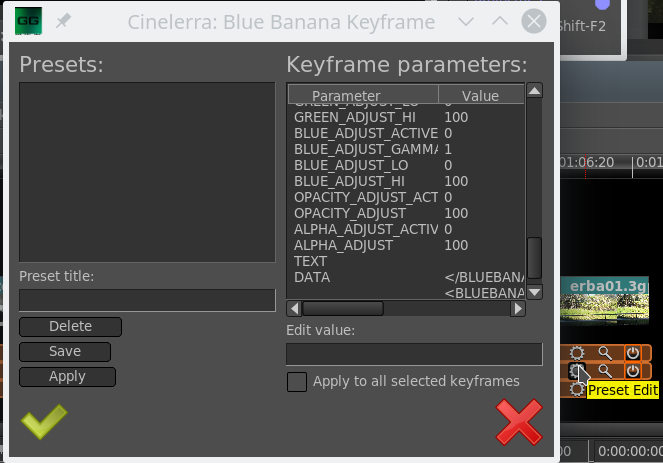
\includegraphics[width=0.8\linewidth]{images/parameters.png}
    \caption{Keyframe Parameters window for a Blue Banana plugin added to the video track}
    \label{fig:parameters}
\end{figure}

\section{Generate Keyframes while Tweaking / Automatic Keyframe Mode}%
\label{sec:generate_keyframe_tweaking}

Tweaking is defined as changing a parameter while playing --- it can be small changes or small motion increments performed in a series.  These changes are recorded as a series of new keyframes on the timeline.  Enable automatic keyframe mode by enabling the automatic keyframe toggle, that is \textit{Generate keyframes while tweaking}.  In automatic keyframe mode, every time you tweak a key-framable parameter it creates a keyframe on the timeline.  Since keyframes affect playback, you should enable generate keyframes just before you need a keyframe and disable when your parameter changes are complete.  So turn on when ready to make changes and turn off when done!

Also, before making a change, be sure to check the View pulldown and make the desired parameter visible with the enable checkmark.  The location where the automatic keyframe is generated is under the insertion point.  If the timeline is playing back during a tweak, several automatic keyframes may be generated as you change the parameter.  When automatic keyframe mode is disabled, adjusting a parameter adjusts the keyframe immediately preceding the insertion point.  For example, if two fade keyframes exist and the insertion point is between them, changing the fader changes the first keyframe.

\section{Compositor Keyframes}%
\label{sec:compositor_keyframes}

Camera and projector translation is represented by two parameters: x and y, making it difficult to adjust with curves.  Cinelerra solves this problem by relying on automatic keyframes.  With a video track loaded, move the insertion point to the beginning of the track and enable automatic keyframe mode.  Move the projector slightly in the compositor window to create a keyframe.  Then go forward several seconds.  Move the projector a long distance to create another keyframe and emphasize motion.  This creates a second projector box in the compositor, with a line joining the two boxes. The joining line is the motion path.  If you create more keyframes, more boxes are created.  Once all the desired keyframes are created, disable automatic keyframe mode.

Dragging the auto curve with tweaking off, adjusts the previous keyframe.  With tweaking on, if no keyframe is at the timeline position, then a new one is created at that position and the modification value is applied.  If you are halfway between two keyframes, the first projector box is adjusted while the second one stays the same.  The video does not appear to move in step with the first keyframe.  This is because halfway between two keyframes, the projector translation is interpolated.  In order to set the second keyframe you will need to move after the second keyframe.

Image translation, motion direction, and speed determine the results.  Motion varies based on the  interpolation type that is set, for example, if set to Linear, the result will be uniform straight line motion.  Smooth is the default so that interpolation will generate curved lines with control points.  Ctrl-drag the endpoint of the control handle to adjust the curved slope.

\section{More about Editing Keyframes}%
\label{sec:more_about_editing_keyframes}

Keyframes can be shifted around and moved between tracks on the timeline using similar cut and paste operations to editing media.  Only the keyframes selected in the View menu are affected by keyframe editing operations. 

An often used, keyframe editing operation is replication of some curve from one track to the other to make a stereo pair.  The first step is to solo the source track's record patch by \texttt{Shift-clicking} on the \textit{arm track} icon in the patchbay.  Then either set In/Out points or highlight the desired region of keyframes.  Go to \texttt{keyframes$\rightarrow$copy keyframes} to copy them to the clipboard.  Solo the destination track's record patch by \texttt{Shift-clicking} on it and go to \texttt{keyframes$\rightarrow$paste keyframes} to paste the clipboard.  Another common application for keyframe modification is to highlight a region on the timeline which contains multiple keyframes that you want to modify.  Then when you adjust a parameter or set of parameters, the change will be applied to all keyframes within the selection instead of a new keyframe being created.  This only works when the keyframe stores multiple parameters and only for mask and effect keyframes.  Other types of keyframes are generated as usual.

And there is an easy way to delete keyframes besides selecting a region and using \texttt{keyframes$\rightarrow$clear keyframes}.  \texttt{Click-drag} a keyframe before its preceding keyframe or after its following keyframe on the track.  This is the only way you can simultaneously delete keyframes on ganged tracks.
